%\RequirePackage[l2tabu, orthodox]{nag}
\documentclass[12pt]{beamer}
\graphicspath{{Imagenes/}{../Imagenes/}}
\usepackage[utf8]{inputenc}
\usepackage[spanish]{babel}
\usepackage[autostyle,spanish=mexican]{csquotes}
\usepackage{hyperref}
\hypersetup{
  colorlinks=true,
  linkcolor=blue,          % color of internal links (change box color with linkbordercolor)
  citecolor=green,        % color of links to bibliography
  filecolor=magenta,      % color of file links
  urlcolor=cyan,           % color of external links
  linkbordercolor={0 0 1}
}
\usepackage{amsmath}
\usepackage{amsthm}
\usepackage{multicol}
\usepackage{graphicx}
\usepackage{physics}
\usepackage{tabulary}
\usepackage{booktabs}
\usepackage[outdir=./]{epstopdf}
%\usepackage{epstopdf}
\usepackage{media9}
\usepackage{multimedia}
\usepackage[binary-units=true]{siunitx}
\usepackage{standalone}
\usepackage{longtable}
\usepackage{bigints}
\usepackage[font=footnotesize,textfont=it]{caption}
%\usepackage{enumitem}
\usepackage{tikz}
\usetikzlibrary{mindmap}
\usepackage[siunitx]{circuitikz}
\usetikzlibrary{arrows, patterns, shapes, decorations.markings, decorations.pathmorphing}
\usetikzlibrary{matrix,positioning}
\tikzstyle{every picture}+=[remember picture,baseline]
\usepackage{color}
\usepackage{alltt}
\usepackage{verbatim}
\usepackage{colortbl}
\usepackage{fancyvrb}
\usepackage[os=win]{menukeys}
\usepackage{pifont}
\usepackage[sfdefault]{roboto}  %% Option 'sfdefault' only if the base font of the document is to be sans serif
%\usepackage[T1]{fontenc}
\setcounter{secnumdepth}{3}
\setcounter{tocdepth}{3}
\DeclareGraphicsExtensions{.pdf,.png,.jpg}
\renewcommand {\arraystretch}{1.5}
\definecolor{ao}{rgb}{0.0, 0.5, 0.0}
\definecolor{bisque}{rgb}{1.0, 0.89, 0.77}
\definecolor{amber}{rgb}{1.0, 0.75, 0.0}
\definecolor{armygreen}{rgb}{0.29, 0.33, 0.13}
\definecolor{alizarin}{rgb}{0.82, 0.1, 0.26}
\definecolor{cadetblue}{rgb}{0.37, 0.62, 0.63}
\newcommand*{\TitleParbox}[1]{\parbox[c]{6cm}{\raggedright #1}}%
\newcommand{\python}{\texttt{python}}
\newcommand{\textoazul}[1]{\textcolor{blue}{#1}}
\newcommand{\azulfuerte}[1]{\textcolor{blue}{\textbf{#1}}}
\newcommand{\funcionazul}[1]{\textcolor{blue}{\textbf{\texttt{#1}}}}
%\normalfont
\usepackage{ccfonts}% http://ctan.org/pkg/{ccfonts}
\usepackage[T1]{fontenc}% http://ctan.or/pkg/fontenc
\renewcommand{\rmdefault}{cmr}% cmr = Computer Modern Roman
\usefonttheme[onlymath]{serif}
\linespread{1.3}
\newcounter{saveenumi}
\newcommand{\seti}{\setcounter{saveenumi}{\value{enumi}}}
\newcommand{\conti}{\setcounter{enumi}{\value{saveenumi}}}
\newcommand{\tikzmark}[1]{\tikz[remember picture] \node[coordinate] (#1) {#1};}

\usepackage{scalerel}[2016-12-29]
\def\stretchint#1{\vcenter{\hbox{\stretchto[440]{\displaystyle\int}{#1}}}}
\def\scaleint#1{\vcenter{\hbox{\scaleto[3ex]{\displaystyle\int}{#1}}}}
\def\bs{\mkern-12mu}

\newtheorem{teo}{}[section]
\usepackage{blkarray}

%reduce el tamaño de letra de la etiqueta equations
\makeatletter
\def\maketag@@@#1{\hbox{\m@th\normalfont\small#1}}
\makeatother

%se usa para la x en itemize
\newcommand{\xmark}{\text{\ding{55}}}

%\AtBeginDocument{\setlength{\tymin}{1em}}


\definecolor{myblue}{rgb}{.8, .8, 1}

\usepackage{amsmath}
\usepackage{empheq}

\newlength\mytemplen
\newsavebox\mytempbox

\makeatletter
\newcommand\mybluebox{%
    \@ifnextchar[%]
       {\@mybluebox}%
       {\@mybluebox[0pt]}}

\def\@mybluebox[#1]{%
    \@ifnextchar[%]
       {\@@mybluebox[#1]}%
       {\@@mybluebox[#1][0pt]}}

\def\@@mybluebox[#1][#2]#3{
    \sbox\mytempbox{#3}%
    \mytemplen\ht\mytempbox
    \advance\mytemplen #1\relax
    \ht\mytempbox\mytemplen
    \mytemplen\dp\mytempbox
    \advance\mytemplen #2\relax
    \dp\mytempbox\mytemplen
    \colorbox{myblue}{\hspace{1em}\usebox{\mytempbox}\hspace{1em}}}

\makeatother



%Se usa la plantilla Warsaw modificada con whale
\mode<presentation>
{
  \usetheme{Warsaw}
  \setbeamertemplate{headline}{}
  %\useoutertheme{infolines}
  \usecolortheme{whale}
  \setbeamercovered{invisible}
  

 \setbeamertemplate{section in toc}[sections numbered]
 \setbeamertemplate{subsection in toc}[subsections numbered]
 \setbeamertemplate{subsection in toc}{\leavevmode\leftskip=3.2em\rlap{\hskip-2em\inserttocsectionnumber.\inserttocsubsectionnumber}\inserttocsubsection\par}
% \setbeamercolor{section in toc}{fg=blue}
 \setbeamercolor{subsection in toc}{fg=blue}
 \setbeamerfont{subsection in toc}{size=\small}


\setbeamertemplate{navigation symbols}{}
\setbeamertemplate{caption}[numbered]
% \setbeamercolor{frametitle}{fg=yellow,bg=blue!70!white}
\setbeamercolor{section in head/foot}{bg=black, fg=white}
%\setbeamercolor{subsection in head/foot}{bg=gray!30,fg=black}
%\setbeamercolor{author in head/foot}{fg=yellow}
%\setbeamercolor{date in head/foot}{fg=blue}

%\mode<presentation>
%{
%  \usetheme{Warsaw}
%  \setbeamertemplate{headline}{}
%  %\useoutertheme{infolines}
%  \useoutertheme{default}
%  \setbeamercovered{invisible}
%  % or whatever (possibly just delete it)
%}
}


\usepackage{courier}
\usepackage{listingsutf8}
\usepackage{listings}
\usepackage{xcolor}
\usepackage{textcomp}
\usepackage{color}
\definecolor{deepblue}{rgb}{0,0,0.5}
\definecolor{brown}{rgb}{0.59, 0.29, 0.0}
\definecolor{OliveGreen}{rgb}{0,0.25,0}
% \usepackage{minted}

\DeclareCaptionFont{white}{\color{white}}
\DeclareCaptionFormat{listing}{\colorbox{gray}{\parbox{0.98\textwidth}{#1#2#3}}}
\captionsetup[lstlisting]{format=listing,labelfont=white,textfont=white}
\renewcommand{\lstlistingname}{Código}


\definecolor{Code}{rgb}{0,0,0}
\definecolor{Keywords}{rgb}{255,0,0}
\definecolor{Strings}{rgb}{255,0,255}
\definecolor{Comments}{rgb}{0,0,255}
\definecolor{Numbers}{rgb}{255,128,0}

\makeatletter

\newif\iffirstchar\firstchartrue
\newif\ifstartedbyadigit
\newif\ifprecededbyequalsign

\newcommand\processletter
{%
  \ifnum\lst@mode=\lst@Pmode%
    \iffirstchar%
        \global\startedbyadigitfalse%
      \fi
      \global\firstcharfalse%
    \fi
}

\newcommand\processdigit
{%
  \ifnum\lst@mode=\lst@Pmode%
      \iffirstchar%
        \global\startedbyadigittrue%
      \fi
      \global\firstcharfalse%
  \fi
}

\lst@AddToHook{OutputOther}%
{%
  \lst@IfLastOtherOneOf{=}
    {\global\precededbyequalsigntrue}
    {}%
}

\lst@AddToHook{Output}%
{%
  \ifprecededbyequalsign%
      \ifstartedbyadigit%
        \def\lst@thestyle{\color{orange}}%
      \fi
    \fi
  \global\firstchartrue%
  \global\startedbyadigitfalse%
  \global\precededbyequalsignfalse%
}

\lstset{ 
language=Python,                % choose the language of the code
basicstyle=\footnotesize\ttfamily,       % the size of the fonts that are used for the code
numbers=left,                   % where to put the line-numbers
numberstyle=\scriptsize,      % the size of the fonts that are used for the line-numbers
stepnumber=1,                   % the step between two line-numbers. If it is 1 each line will be numbered
numbersep=5pt,                  % how far the line-numbers are from the code
backgroundcolor=\color{white},  % choose the background color. You must add \usepackage{color}
showspaces=false,               % show spaces adding particular underscores
showstringspaces=false,         % underline spaces within strings
showtabs=false,                 % show tabs within strings adding particular underscores
frame=single,   		% adds a frame around the code
tabsize=2,  		% sets default tabsize to 2 spaces
captionpos=t,   		% sets the caption-position to bottom
breaklines=true,    	% sets automatic line breaking
breakatwhitespace=false,    % sets if automatic breaks should only happen at whitespace
escapeinside={| |},  % if you want to add a comment within your code
stringstyle =\color{OliveGreen},
otherkeywords={as, np.array, np.concatenate, np.linspace, linspace, interpolate.interp1d, kind, plt.plot, .copy, np.arange, np.cos, np.pi, lw, ls, label, splrep, splev, plt.legend, loc, plt.title, plt.ylim, plt.show, sign, math.ceil, math.log, np.sqrt, np.exp, np.zeros, plt.xlabel, plt.ylabel, plt.xlim, np.identity, random, np.dot, np.outer, np.diagonal },             % Add keywords here
keywordstyle = \color{blue},
commentstyle = \color{darkcerulean},
identifierstyle = \color{black},
literate=%
         {á}{{\'a}}1
         {é}{{\'e}}1
         {í}{{\'i}}1
         {ó}{{\'o}}1
         {ú}{{\'u}}1
%
%keywordstyle=\ttb\color{deepblue}
%fancyvrb = true,
}

\lstdefinestyle{FormattedNumber}{%
    literate={0}{{\textcolor{red}{0}}}{1}%
             {1}{{\textcolor{red}{1}}}{1}%
             {2}{{\textcolor{red}{2}}}{1}%
             {3}{{\textcolor{red}{3}}}{1}%
             {4}{{\textcolor{red}{4}}}{1}%
             {5}{{\textcolor{red}{5}}}{1}%
             {6}{{\textcolor{red}{6}}}{1}%
             {7}{{\textcolor{red}{7}}}{1}%
             {8}{{\textcolor{red}{8}}}{1}%
             {9}{{\textcolor{red}{9}}}{1}%
             {.0}{{\textcolor{red}{.0}}}{2}% Following is to ensure that only periods
             {.1}{{\textcolor{red}{.1}}}{2}% followed by a digit are changed.
             {.2}{{\textcolor{red}{.2}}}{2}%
             {.3}{{\textcolor{red}{.3}}}{2}%
             {.4}{{\textcolor{red}{.4}}}{2}%
             {.5}{{\textcolor{red}{.5}}}{2}%
             {.6}{{\textcolor{red}{.6}}}{2}%
             {.7}{{\textcolor{red}{.7}}}{2}%
             {.8}{{\textcolor{red}{.8}}}{2}%
             {.9}{{\textcolor{red}{.9}}}{2}%
             {\ }{{ }}{1}% handle the space
         ,%
          %mathescape=true
          escapeinside={__}
          }



\makeatletter

% \setbeamercolor{subsection in foot}{bg=blue!30!yellow, fg=red}
%\setbeamercolor{footlinecolor}{bg=black,fg=white}
\setbeamertemplate{footline}
{
  \leavevmode%
  \hbox{%
  \begin{beamercolorbox}[wd=.333333\paperwidth,ht=2.25ex,dp=1ex,center]{section in footline}%
    \usebeamerfont{section in foot} \insertsection
  \end{beamercolorbox}}%
  \begin{beamercolorbox}[wd=.333333\paperwidth,ht=2.25ex,dp=1ex,center]{subsection in foot}%
    \usebeamerfont{subsection in foot}  \insertsubsection
  \end{beamercolorbox}%
  \begin{beamercolorbox}[wd=.333333\paperwidth,ht=2.25ex,dp=1ex,right]{date in head/foot}%
    \usebeamerfont{date in head/foot} \insertshortdate{} \hspace*{2em}
    \insertframenumber{} / \inserttotalframenumber \hspace*{2ex} 
  \end{beamercolorbox}}%
  \vskip0pt%
\makeatother
\normalfont
\usepackage{ccfonts}% http://ctan.org/pkg/{ccfonts}
\usepackage[T1]{fontenc}% http://ctan.or/pkg/fontenc
\renewcommand{\rmdefault}{cmr}% cmr = Computer Modern Roman
\linespread{1.3}
\title{Ecuaciones diferenciales ordinarias}
\subtitle{Curso de Física Computacional}
\author{M. en C. Gustavo Contreras Mayén}
\date{\today}
\institute{Facultad de Ciencias - UNAM}
\titlegraphic{
\includegraphics[width=1.75cm]{Imagenes/escudo-facultad-ciencias.jpg}\hspace*{4.75cm}~%
   
\includegraphics[width=1.75cm]{Imagenes/escudo-unam.jpg}
}
\begin{document}
\maketitle
\fontsize{14}{14}\selectfont
\spanishdecimal{.}
\section*{Contenido}
\frame{\tableofcontents[currentsection, hideallsubsections]}
\section{Ecuaciones Diferenciales Ordinarias}
\frame{\tableofcontents[currentsection, hideothersubsections]}
\subsection{Introducción}
\begin{frame}
\frametitle{Introducción.}
Las ecuaciones diferenciales tienen importancia fundamental en las aplicaciones, ya que muchas leyes y relaciones físicas pueden expresarse matemáticamente de esta forma.
\\
\medskip
En particular, el estudio de problemas de equilibrio de sistemas continuos se encuentra dentro de este contexto.
\end{frame}
\begin{frame}
\frametitle{Definiciones importantes}
\begin{block}{Aviso de consideración}
	No sería mala idea hacer un repaso en casa sobre estas definiciones y los métodos analíticos de solución de las	 \textit{Ecuaciones Diferenciales Ordinarias} EDO.
\end{block}
\end{frame}
\begin{frame}
\frametitle{Ecuación diferencial}
Esta ecuación relaciona dos o más variables en términos de derivadas o diferenciales.
\\
%\fontsize{12}{12}\selectfont
\begin{align*}
\dfrac{dy}{dx} & =  \cos x \\
\dfrac{d^{2} y}{dx^{2}} & =   \cos x \\
( x^{2} + y^{2} ) dx + 2 xy dy & =  0 \\
\left[ \dfrac{x^{2} w}{dx^{2}} \right]^{3} - xy \dfrac{dw}{dx} & = 0 
\end{align*}
\end{frame}
\begin{frame}
\frametitle{EDO y EDP}
Si en una ecuación diferencial hay una sola variable independiente, las derivadas son totales y se le llama \textcolor{blue}{\textit{ecuación ordinaria}}.
\\
\medskip
\pause
Si en la ecuación hay dos o más variables independientes, las derivadas serán parciales y se le llama \textcolor{red}{\textit{ecuación parcial}}.
\[ \dfrac{\partial^{2} V}{\partial x^{2}} + \dfrac{\partial^{2} V}{\partial y^{2}} = 0\]
\end{frame}
\begin{frame}
\frametitle{Orden de una ecuación diferencial}
Es la derivada de mayor orden que aparece en la ecuación.
\end{frame}
\begin{frame}
\frametitle{Grado de una ecuación diferencial}
Es el grado \textit{algebraico} de la derivada de mayor orden que aparece en la ecuación.
\end{frame}
\begin{frame}
\frametitle{Ecuación diferencial lineal}
Una ecuación diferencial es lineal si en ella no aparecen potencias de la variable dependiente y sus derivadas, ni productos de la variable dependiente por sus derivadas o productos entre derivadas.
\end{frame}
\begin{frame}
\frametitle{Solución de una ecuación diferencial}
Es cualquier relación funcional que no incluya derivadas o integrales de funciones desconocidas y que implique a la propia ecuación diferencial, en el sentido de que la verifique por sustitución directa.
\end{frame}
\begin{frame}
\frametitle{Ecuación y condiciones homogéneas}
Una ecuación o condición es homogénea si, cuando es satisfecha por una función particular $y(x)$, también es satisfecha por $c \; y(x)$, donde $c$ es una constante arbitraria.
\end{frame}
\begin{frame}
\frametitle{Solución de una ecuación diferencial}
Sea una ecuación diferencial ordinaria de orden $n$ y cualquier grado, cuya forma más general es:
\[F(x, y, y^{\prime}, y^{\prime \prime}, \ldots, y^{(n)}) = 0\]
Se establece del cálculo que en su solución general deben de aparecer $n$ constantes arbitrarias. Entonces puede aceptarse como solución general:
\[G(x, y, c_{1}, c_{2}, \ldots, c_{n}) = 0\]
\end{frame}
\begin{frame}[fragile]
\frametitle{Solución de una EDO}
\begin{figure}
	\centering
	\includestandalone{Figuras/fig_edo_01}
	\caption{Familia de curvas planas para cada constante $n$}
\end{figure}
\end{frame}
\begin{frame}
\frametitle{Ejemplo}
Gráficamente esta ecuación representa a una familia de curvas planas, cada una de ellas obtenidas para valores particulares de las $n$ constantes $c_{1}, c_{2}, \ldots, c_{n}$
\end{frame}
\begin{frame}
\frametitle{Tipos de problemas}
Dependiendo de cómo se establezcan estas condiciones, se distinguen dos tipos de problemas los llamados {\color{red}\textit{de valores iniciales}} y los {\color{red}\textit{de valores en la frontera}}.
\end{frame}
\begin{frame}
\frametitle{Problemas de valores iniciales}
Está gobernado por una ecuación diferencial de orden $n$ y un conjunto de $n$ condiciones independientes, todas ellas válidas para el mismo punto inicial.
\\
\medskip
Si la ecuación diferencial que define el problema es del tipo de la EDO con la que iniciamos y $x=a$ es el punto inicial, puede aceptarse que las $n$ condiciones independientes son:
\end{frame}
\begin{frame}
\frametitle{$n$ condiciones independientes}
\begin{align*}
y(a) & = y_{0} \\
y^{\prime}(a) & = y^{\prime}_{0} \\
y^{\prime \prime}(a) & = y^{\prime \prime}_{0} \\
\vdots \\
y^{n}(a) & = y^{n}_{0}
\end{align*}
Y se tratará de obtener una solución particular de la EDO inicial que verifique las condiciones iniciales, como se presenta en la siguiente figura:
\end{frame}
\begin{frame}[fragile]
\frametitle{Solución de EDO con condiciones inciales}
\begin{figure}
	\centering
	\includestandalone{Figuras/fig_edo_02}
	\caption{Solución de la EDO con una condición inicial.}
\end{figure}
\end{frame}
\begin{frame}
\frametitle{Problemas de valores en la frontera}
Se deben de establecer condiciones de frontera en todos y cada uno de los puntos que constituyen la frontera del dominio de soluciones del problema.
\end{frame}
\begin{frame}
\frametitle{Problemas de valores en la frontera}
En particular, en el espacio de una dimensión, hay dos puntos frontera, por ejemplo $x=a$ y $x=b$ si el dominio de soluciones es el intervalo cerrado $a \leq x \leq b$
\end{frame}
\begin{frame}[fragile]
\frametitle{Solución de EDO con condiciones de frontera}
\begin{figure}
	\centering
	\includestandalone{Figuras/fig_edo_03}
	\caption{Solución de la EDO con condiciones de frontera.}
\end{figure}
\end{frame}
\begin{frame}
\frametitle{Estrategia de solución}
Básicamente la solución numérica de las ecuaciones diferenciales consiste en sustituir el dominio continuo de soluciones por uno discreto formado por puntos aislados igualmente espaciados entre sí.
\end{frame}
\begin{frame}
\frametitle{Problema de valores iniciales}
El dominio de definición de soluciones $x \geq a$  se sustituye por el conjunto infinito numerable de puntos:
\begin{align*}
x_{0} & = a \\
x_{1} & = x_{0} + h \\
x_{2} & = x_{0} + 2h \\
x_{3} & = x_{0} + 3h \\
\ldots
\end{align*}
\end{frame}
\begin{frame}[fragile]
\frametitle{Valores inciales}
\begin{figure}
	\centering
	\includestandalone{Figuras/fig_edo_04}
	\caption{Solución de la EDO con valores iniciales.}
\end{figure}
\end{frame}
\begin{frame}
\frametitle{Problema de valores en la frontera}
Se sustituye el intervalo $a \leq x \leq b $ por el conjunto finito de puntos:
\begin{align*}
x_{0} & = a \\
x_{1} & = x_{0} + h \\
x_{2} & = x_{0} + 2 \; h \\
x_{3} & = x_{0} + 3 \; h \\
\ldots \\
x_{n} & = x_{0} + n \;h = b
\end{align*}
\end{frame}
\begin{frame}[fragile]
\frametitle{Valores en la frontera}
\begin{figure}
	\centering
	\includestandalone{Figuras/fig_edo_05}
	\caption{Solución con valores en la frontera.}
\end{figure}
\end{frame}
\begin{frame}
\frametitle{Nuestra tarea}
Habiéndose discretizado el problema continuo, se tratará de obtener la solución para los puntos considerados, esto se resuelve en general, de dos maneras:
\end{frame}
\begin{frame}
\frametitle{Nuestra tarea}
\setbeamercolor{item projected}{bg=red!70!black,fg=white}
\setbeamertemplate{enumerate items}[circle]
\begin{enumerate}[<+->]
\item Sustituyendo las derivadas que aparezcan en la ecuación diferencial y en sus condiciones iniciales o de frontera, por fórmulas numéricas de derivación que proporcionen una aproximación a las derivadas.
\item Tratando de integrar la ecuación, reemplazando el proceso de integración por una fórmula numérica que se aproxime a la integral.
\end{enumerate}
\end{frame}
\section{Problemas de valores iniciales}
\frame{\tableofcontents[currentsection, hideothersubsections]}
\subsection{Definición de PVI}
\begin{frame}
\frametitle{Problemas de valores iniciales}
Debemos de resolver
\[ y^{\prime} = F(x, y)\]
con la condición auxiliar $y(a) = \alpha$
\end{frame}
\begin{frame}
\frametitle{Forma general de una EDO de 1er. orden}
La forma general de una ecuación diferencial de primer orden (1-EDO) es
\[ y^{\prime} = f(x, y) \]
donde $y^{\prime} = dy/dx$ y $f(x, y)$ es una función dada.
\\
\bigskip
La solución de esta ecuación incluye una constante arbitraria (la constante de integración)
\end{frame}
\begin{frame}
\frametitle{Constante de integración}
Para hallar esa constante, debemos conocer un punto en la curva solución, esto es, $y$ debe de especificarse para algún valor de $x$, $x = a$.
\\
\bigskip
Entonces, escribimos, la condición auxiliar $y(a) = \alpha$
\end{frame}
\begin{frame}
\frametitle{Transformación de una EDO de orden $n$}
Una ecuación diferencial de orden $n$
\[y^{(n)} = f(x, y, y^{\prime}, \ldots, y^{(n - 1)})\]
se puede transformar en un conjunto de $n$ ecuaciones diferenciales de primer orden.
\end{frame}
\begin{frame}
\frametitle{Ajuste en la notación}
Usemos la siguiente notación
\begin{align*}
y_{0} & =y \\
y_{1} & = y^{\prime} \\
y_{2} & =y^{\prime \prime} \\
\ldots \\
y_{n - 1} &= y^{(n - 1)}
\end{align*}
\end{frame}
\begin{frame}
\frametitle{Sistema de 1-EDO}
Las ecuaciones diferenciales ordinarias de primer orden (\textcolor{blue}{1-EDO}) equivalentes son:
\begin{align*}
y^{\prime}_{0} & =y_{1} \\
y^{\prime}_{1} & = y_{2} \\
y^{\prime}_{2} & = y_{3} \\
\ldots \\
y^{\prime}_{n} & = f(x, y_{0}, y_{1}, \ldots, y_{n-1})
\end{align*}
\end{frame}
\begin{frame}
\frametitle{Solución con $n$ condiciones iniciales}
La solución ahora requiere de $n$ condiciones iniciales; si esas condiciones se especifican para el mismo valor de $x$, el problema se dice que es \emph{un problema de valores iniciales}.
\\
\medskip
Las \emph{condiciones iniciales}, tienen la forma:
\[ y_{0}(a) = \alpha_{0}, \hspace{0.75cm} y_{1}(a) = \alpha_{1}, \hspace{0.75cm} \ldots \hspace{0.75cm} y_{n - 1}(a) = \alpha_{n-1}\]
\end{frame}
\begin{frame}
\frametitle{Problemas de valores iniciales}
Si $y_{i}$ se especifica para diferentes valores de $x$, el problema se llama \emph{problema con condiciones de frontera}, por ejemplo:
\[ y^{\prime \prime} = -y \hspace{1cm} y(0)=1 \hspace{1cm} y^{\prime}(0) = 0\]
es un problema de condiciones iniciales, ya que ambas condiciones están definidas en la solución para $x = 0$
\end{frame}
\begin{frame}
\frametitle{Problemas con valores en la frontera}
En cambio el problema
\[ y^{\prime \prime} = - y \hspace{1cm} y(0) = 1 \hspace{1cm} y^{\prime}(\pi) = 0\]
es un problema con condiciones de frontera, ya que las dos condiciones se cumplen para diferentes valores de $x$.
\end{frame}
\begin{frame}
\frametitle{Notación usada para el tema EDO}
Se usará de manera continua y por conveniencia, la notación vectorial, que nos permitirá manejar conjuntos de \textcolor{blue}{1-EDO} de una manera más clara, de tal manera que podremos expresar:
\[ \mathbf{y}^{\prime} = \mathbf{F}(x,\mathbf{y}) \hspace{1.3cm} \mathbf{y}(a) = \alpha\]
\[ \mathbf{F}(x,\mathbf{y}) = \left[ \begin{matrix}
y_{1} \\
y_{2} \\
\ldots \\
f(x,\mathbf{y})
\end{matrix} \right] \]
\end{frame}
\subsection{Método de Euler (serie de Taylor)}
\begin{frame}
\frametitle{Método de Euler (serie de Taylor)}
El método de la Serie de Taylor es sencillo conceptualmente y con una mayor precisión.
\\
\medskip
Se basa en la serie de Taylor truncada para $y$ alrededor de $x$:
\[ y(x+h) \simeq y(x) + y'(x) h  \]
\end{frame}
\begin{frame}
La fórmula anterior predice el valor de $y$ en $x+h$ con la información disponible de $x$, se puede utilizar para mover la solución hacia adelante en incrementos de $h$, para los valores iniciales de $x$ y de $y$.
\end{frame}
\begin{frame}
\frametitle{Error de truncamiento}
El error debido al truncamiento, es:
\[ E = \dfrac{1}{2} \: y^{\prime \prime} (\xi) \:  h^{2} = O(h^{2}), \hspace{1cm} x < \xi < x + h \]
\end{frame}
\begin{frame}
\frametitle{Método de Euler}
Para simplificar, consideremos que tenemos una sola variable $y$, y que la ecuación diferencial es $y^{\prime} = f(x, y)$.
\begin{figure}
	\centering
	\includestandalone{fig_edo_06}
	\caption{Representación gráfica del método de Euler.}
\end{figure}
\end{frame}
\begin{frame}
El cambio en la solución $y$ entre $x$ y $x + h$ es
\[ y(x + h) - y(h) = \int_{x}^{x + h} \: y^{\prime} \: dx = \int_{x}^{x + h} \: f(x, y) \: dx \]
que es el área debajo de la gráfica de $y^{\prime}(x)$.
\end{frame}
\begin{frame}
La fórmula de Euler aproxima ésta área con el área del rectángulo sombreado. El área entre el rectángulo sombreado y la gráfica representa el error debido al truncamiento.
\begin{figure}
	\centering
	\includestandalone{fig_edo_06}
	\caption{Aproximación del área debajo de la curva.}
\end{figure}
\end{frame}
\begin{frame}
Se revisa claramente que el error de truncamiento es proporcional a la pendiente de la gráfica, esto es, proporcional a $y'(x)$
\begin{figure}
	\centering
	\includestandalone{fig_edo_06}
	\caption{El error debido al truncamiento es proporcional a la derivada.}
\end{figure}
\end{frame}
\begin{frame}
El método de Euler rara vez se utiliza en la práctica debido a su ineficiencia computacional.
\\
\bigskip
Para reducir el error de truncamiento a un nivel aceptable, \textcolor{blue}{requiere considerar un valor de $h$ muy pequeño}, dando lugar a muchos pasos de integración acompañados por un incremento en el error de redondeo.
\end{frame}
\begin{frame}
El valor del método de Euler radica principalmente en su simplicidad, lo que facilita la discusión de ciertos temas importantes, como la estabilidad.
\end{frame}
\subsection{La función \texttt{euler}}
\begin{frame}
\frametitle{La función \texttt{euler}}
Vamos a construir una función que use el método de integración de Euler.
\\
\medskip
La función puede manejar cualquier número de ecuaciones diferenciales de primer orden. 
\\
\bigskip
El usuario debe proporcionar la función $F(x, y)$ que especifica las ecuaciones diferenciales en el formato de un arreglo.
\end{frame}
\begin{frame}
\frametitle{La función \texttt{euler}}
Arreglo para las \textcolor{blue}{1-EDO}
\[ \mathbf{F}(x,y) =
\begin{bmatrix}
y^{\prime}_{0} \\
y^{\prime}_{1} \\
y^{\prime}_{2} \\
\vdots
\end{bmatrix} \]
La función devuelve los arreglos $X$ y $Y$ que contienen los valores de $x$, de $y$ en intervalos de tamaño $h$.
\end{frame}
\begin{frame}[fragile]
\begin{lstlisting}[caption=La función euler, style=FormattedNumber, basicstyle=\linespread{1.1}\ttfamily=\small, columns=fullflexible]
def euler(F, x, y, xAlto, h):
    X = []
    Y = []

    X.append(x)
    Y.append(y)
    
    while x < xAlto:
        h = min(h, xAlto - x)
        y = y + h * F(x, y)
        x = x + h
        X.append(x)
        Y.append(y)
   
   return np.array(X), np.array(Y)
\end{lstlisting}
\end{frame}
\begin{frame}
\frametitle{Rutinas para visualizar los resultados}
A continuación se presentan dos rutinas que nos ayudarán a visualizar mejor los resultados en pantalla. Usaremos la función \azulfuerte{\texttt{imprimeSoln}} para imprimir los arreglos $X$ y $Y$ obtenidos de la integración numérica. 
\end{frame}
\begin{frame}
\frametitle{Rutinas para visualizar los resultados}
La cantidad de datos se controla con el parámetro \texttt{freq}:
\begin{itemize}[<+->]
\item Si \texttt{freq = 5}: se presentará el valor obtenido cada cinco pasos.
\item Si \texttt{freq = 0}, sólo se presentan el valor inicial y el final.
\end{itemize}
\end{frame}
\begin{frame}[plain, allowframebreaks, fragile]
\begin{lstlisting}[caption=Función para visualizar los datos, style=FormattedNumber, basicstyle=\linespread{1.1}\ttfamily=\small, columns=fullflexible]
def imprimeSoln(X,Y,freq):
   
   def imprimeEncabezado(n):
       print ('\n x ')
       for i in range (n):
           print (' y[',i,']')
       print()
    
    def imprimeLinea(x,y,n):
        print ("{:_13_._4_e}".format(x))
        for i in range (n):
            print ("{:_13_._4_e}".format(y[i]))
            print()

    m = len(Y)
    try: n = len(Y[_0_])
    except TypeError: n = 1
    if freq == 0: freq = m

    imprimeEncabezado(n)
    for i in range(0, m, freq):
        imprimeLinea(X[i], Y[i],n)
    if i != m - 1: imprimeLinea(X[m - _1_], Y[m - _1_], n)
\end{lstlisting}
\end{frame}
\subsection{Ejercicio 1}
\begin{frame}
\frametitle{Ejercicio 1}
Resolver
\[ y^{\prime \prime} = -0.1 \: y^{\prime} - x \hspace{0.75cm} y(0) = 0 \hspace{0.5cm} y^{\prime} (0) = 1\]
de $x = 0$ hasta $x = 2$ con el método de Euler, usa $h = 0.05$, grafica el valor de $y$ así como la solución analítica
\[ y = 100 \; x - 5 \; x^{2} + 990 (e^{-0.1 \; x} - 1 ) \]
\end{frame}
\begin{frame}
\frametitle{Solución}
Usemos la notación $y_{0} = y$ y $y_{1} = y^{\prime}$ para un conjunto de \textcolor{blue}{1-EDO} equivalentes y las condiciones iniciales
\[\mathbf{F(x, y)} = 
\begin{bmatrix}
y^{\prime}_{0} \\
y^{\prime}_{1}
\end{bmatrix} =
\begin{bmatrix}
y_{1} \\
-0.1 y_{1} - x
\end{bmatrix}
\hspace{1.5cm}
\mathbf{y}(0) = 
\begin{bmatrix}
0 \\
1
\end{bmatrix} \]
\end{frame}
\begin{frame}[plain, allowframebreaks, fragile]
\begin{lstlisting}[caption=Código para el Ejercicio, style=FormattedNumber, basicstyle=\linespread{1.1}\ttfamily=\small, columns=fullflexible]
from numpy import zeros, array, exp, linespace

def F(x, y):
    F = zeros(2)
    F[_0_] = y[_1_]
    F[_1_] = -0.1 * y[_1_] - x
    return F
	
x = 0.0
xAlto = 2.0

y = array([0.0, 1.0])
h = 0.05

freq = 1

X, Y = euler(F, x, y, xAlto, h)

imprimeSoln(X, Y, freq)
\end{lstlisting}
\end{frame}
\begin{frame}[allowframebreaks, plain, fragile]
\frametitle{Código para evaluar la solución}
Para comparar los resultados, se necesita evaluar en el dominio $x$, la función que representa la solución, entonces:
\begin{lstlisting}[caption=Código que evalúa la solución, style=FormattedNumber, basicstyle=\linespread{1.1}\ttfamily=\small, columns=fullflexible]
x = linspace(-2, 2, 100)

def yExacta(x):
	return 100.0 * x - 5.0 * x**2 + 990.0 * (exp(-0.1 * x) - 1.0)

plt.plot(x, yExacta(x), 'k', label='Exacta')
plt.show()
\end{lstlisting}
\end{frame}
\begin{frame}
\frametitle{Graficar la solución de la EDO}
Nos resta generar la gráfica para la solución con los arreglos $X$, $Y$ que obtenemos de la función \funcionazul{euler}, pero recordemos que el arreglo $Y$ contiene n-elementos que a su vez son arreglos: $Y[0], Y[1], \ldots, Y[n-1], Y[n]$.
\end{frame}
\begin{frame}[allowframebreaks, plain, fragile]
\frametitle{Seleccionando el arreglo $Y[0]$}
Como sólo nos interesa mostrar la solución, es decir: $y$, debemos de seleccionar ese elemento, para ello, usamos el \emph{slicing} de los arreglos:
\begin{lstlisting}[caption=Código para graficar la solución de la EDO, style=FormattedNumber, basicstyle=\linespread{1.1}\ttfamily=\small, columns=fullflexible]
plt.plot(X, Y[:,0], 'bo', label=' Solucion euler')
plt.show()
\end{lstlisting}
\end{frame}
\begin{frame}[fragile]
\frametitle{Gráfica con la solución numérica y la exacta}
\begin{figure}
	\centering
	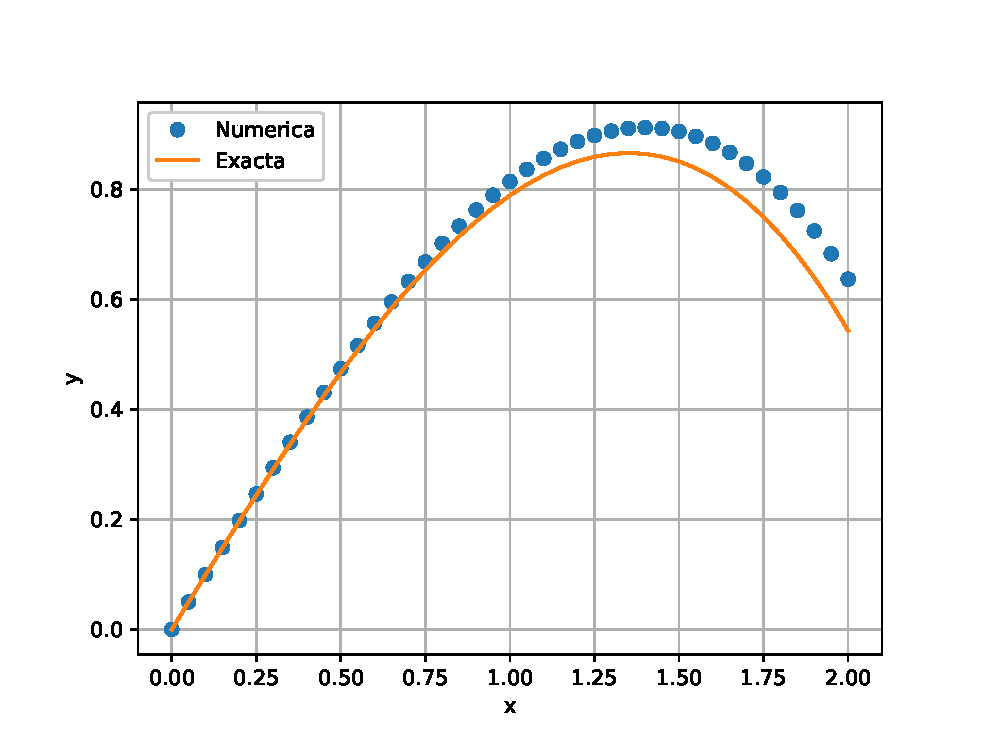
\includegraphics[scale=0.6]{sol_edo_01.eps}
\end{figure}
\end{frame}
\begin{frame}
\frametitle{¿Por qué usamos $Y[:,0]$}
Lo que nos devuelve la función \funcionazul{euler} son los arreglos $X$, $Y$, éste último es un arreglo que contiene arreglos, es decir:
\[  Y = [Y[0], \hspace{0.2cm} Y[1], , \ldots, Y[n-1], \hspace{0.2cm} Y[n] ] \]
A este manejo de arreglos, se le denomina \textoazul{arreglos anidados}.
\end{frame}
\begin{frame}
\frametitle{Listas anidadas}
Cada arreglo $Y[0]$, \ldots $Y[n]$ está conformado por dos elementos:
\begin{align*}
Y[0] &= [Y[0][0], Y[0][1] ] \\
Y[1] &= [Y[1][0], Y[1][1] ] \\
Y[2] &= [Y[2][0], Y[2][1] ] \\
\vdots \\
Y[n - 1] &= [Y[n - 1][0], Y[n -1 ][1] ] \\
Y[n] &= [Y[n][0], Y[n][1] ]
\end{align*}
Podemos manejar un elemento en particular de los arreglos, usando los respectivos índices.
\end{frame}
\begin{frame}[fragile]
\frametitle{Elementos de $Y$}
Lo que contiene el arreglo $Y$ es lo siguiente:
\begin{verbatim}
[[ 0.          1.        ]
 [ 0.05        0.995     ]
 [ 0.09975     0.987525  ]
 ...
 [ 0.72445689 -0.82994569]
 [ 0.68295961 -0.92079596]
 [ 0.63691981 -1.01369198]]
 \end{verbatim}
\end{frame}
\begin{frame}
\frametitle{Recuperando un arreglo completo}
Necesitamos todos los valores $Y[i][0]$ del arreglo $Y$, que representan la solución de la EDO, entonces usamos el \emph{slicing}: \textoazul{\texttt{Y[:,0]}}, que debemos de interpretar:
\\
\bigskip
\emph{Dame todos los elementos de las listas cuyo segundo índice sea cero} = $Y[i][0]$, la coma es necesaria para separar el segundo índice.
\end{frame}
\begin{frame}
\frametitle{Elemento recuperado para graficar}
Ahora ya contamos con una lista con el mismo número de elementos que la lista $X$ (tienen la misma dimensión), ya podemos usarlo en la instrucción de graficación.
\end{frame}
% \section{Métodos de Runge-Kutta}
% \frame{\tableofcontents[currentsection, hideothersubsections]}
% \subsection{Definición de RK}
% \begin{frame}
% \frametitle{Métodos de Runge-Kutta}
% La principal desventaja del método de Euler es que su precisión es baja. 
% \\
% \bigskip
% Para hacer que el nivel de precisión aumente, hay que reducir $h$, pero esto genera que se lleve más tiempo en el cálculo y se propague el error por redondeo.
% \end{frame}
% \begin{frame}
% Sea una EDO:
% \[y^{\prime} =  f(y,t), \hspace{1cm y(0)= y_{0}}\]
% Para calcular $y_{n+1} = t_{n} + h$ dando un valor de $y_{n}$ se integra la EDO en el intervalo $[t_{n}, t_{n+1}]$
% \[y_{n + 1} = y_{n} + \int_{t_{n}}^{t_{n + 1}} \: f(y,t) dt\]
% Se resuelve la ecuación del lado derecho mediante integración numérica.
% \end{frame}
% \subsection{Runge-Kutta de segundo orden}
% \begin{frame}
% \frametitle{Runge-Kutta de segundo orden}
% Aplicando la regla del trapecio al lado derecho de la ecuación anterior:
% \[\int_{t_{n}}^{t_{n+1}} f(y,t) dt \simeq \dfrac{1}{2} h [f(y_{n},t_{n}) + f(y_{n+1}, t_{n+1})] \]
% En esta ecuación el término $y_{n+1}$ es una incógnita, por lo que se aproxima el segundo término mediante $f(y*_{n+1},t_{n+1})$ donde $y*_{n+1}$ es la primera estimación de $y_{n+1}$ obtenido por el método de Euler hacia adelante.
% \end{frame}
% \begin{frame}
% \begin{eqnarray*}
% y*_{n+1} & = & y_{n} + h f(y_{n},t_{n}) \\
% y_{n+1} & = & y_{n} + \dfrac{h}{2} [f(y_{n},t_{n}) + f(y*_{n+1},t_{n+1})]
% \end{eqnarray*}
% De manera canónica, podemos escribir:
% \begin{eqnarray*}
% k_{1} & = & h f(y_{n},t_{n}) \\
% k_{2} & = & h f(y_{n} + k_{1}, t_{n+1})\\
% y_{n+1} & = & y_{n} + \dfrac{1}{2}[k_{1}+k_{2}]
% \end{eqnarray*}
% \end{frame}
% \begin{frame}[fragile]
% \frametitle{Ejercicio}
% El circuito que se muestra, tiene una autoinductancia de $L = \SI{50}{\henry}$, una resistencia de $R = \SI{20}{\ohm}$, y una fuente de $V = \SI{10}{\volt}$.
% \begin{figure}
%     \centering
%     \includestandalone{Figuras/circuito_RK2}
%     \caption{Circuito RLC para el ejercicio.}
% \end{figure}
% \end{frame}
% \begin{frame}
% En el tiempo $t = 0$, la corriente $I(t)$ satisface
% \[L \dfrac{d}{dt} I(t) + RI(t) = V, \hspace{1cm} I(0) = 0\]
% Usando el esquema de Runge-Kutta de segundo orden (RK2), calcula la corriente en el circuito para $0\leq t \leq 10$ segundos, con $h=0.1$
% \end{frame}
% \begin{frame}
% Se reescribe la ecuación como
% \[\dfrac{d}{dt} I = -\dfrac{R}{L} I + \dfrac{V}{L} = f(I,t)\]
% Aplicando el método RK2, tenemos
% \begin{eqnarray*}
% k_{1} &=& h \left[-\dfrac{R}{L} I_{n} + \dfrac{V}{L} \right] \\
% k_{2} &=& h \left[-\dfrac{R}{L} (I_{n}+k_{1}) + \dfrac{V}{L} \right] \\
% I_{n+1} &=& I_{n} + \dfrac{1}{2} (k_{1} + k_{2})
% \end{eqnarray*}
% \end{frame}
% \begin{frame}[fragile]
% \fontsize{10}{10}\selectfont
% \begin{lstlisting}[caption=Código para el Ejercicio, style=FormattedNumber, basicstyle=\linespread{1.1}\ttfamily=\small, columns=fullflexible]
% L = 50.0
% R = 20.0
% V = 10.0
% h = 0.1
% corriente = 0
% I = []
% I.append(0)

% for i in range(99):
%     k_1_ = h * ((-R/L) * corriente + (V/L))
%     k_2_ = h *((-R/L) * (corriente + k_1_) + (V/L))
%     corriente = corriente + (k_1_ + k_2_) * 0.5
%     I.append(corriente)
% \end{lstlisting}
% \end{frame}
% \begin{frame}
% La rutina para la gráfica con \azulfuerte{\texttt{matplotlib}} la pueden implementar sin mayor problema.
% \\
% \bigskip
% Nótese que el valor de corriente límite corresponde a $I_{f}=V/R$ que alcanzaría en un tiempo mucho mayor.
% \end{frame}
% \begin{frame}[fragile]
% \frametitle{Resultado gráfico}
% \begin{figure}
% 	\centering
% 	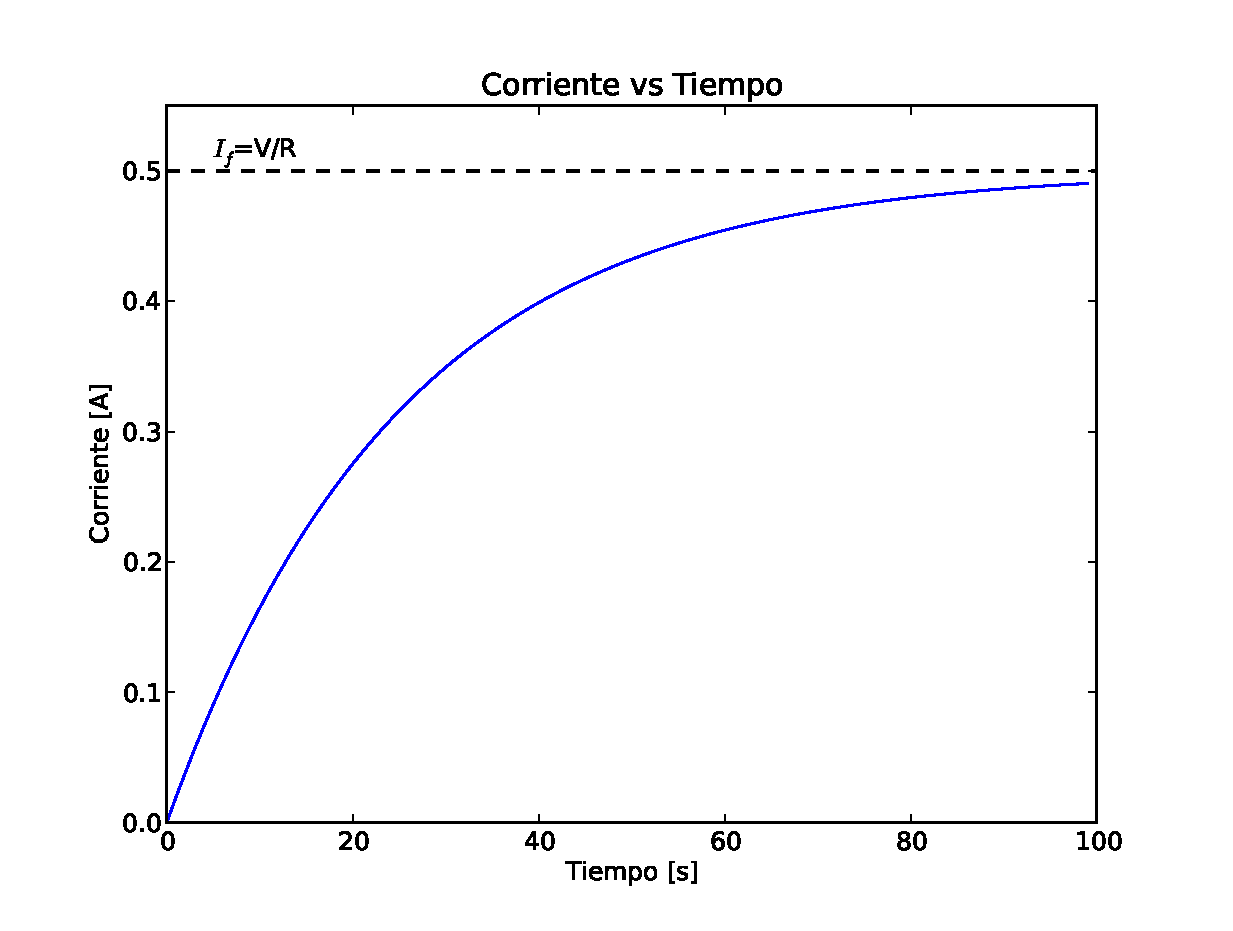
\includegraphics[scale=0.4]{Imagenes/RK2circuito.eps} 
%     \caption{Solución para el circuito, la corriente llega a un límite definido por el valor de $V$ y de $R$.}
% \end{figure}
% \end{frame}
% \begin{frame}
% El objetivo de los métodos de Runge-Kutta (RK) es eliminar la necesidad de la diferenciación repetida de las ecuaciones diferenciales. 
% \\
% \medskip
% Dado que la diferenciación repetida no está implicada en la fórmula de integración en serie de Taylor de primer orden
% \[ \mathbf{y}(x+h) = \mathbf{y}(x) + \mathbf{y}^{\prime}(x) \: h = \mathbf{y}(x) + \mathbf{F}(x,\mathbf{y}) \: h \]
% Se considera como el método Runge-Kutta de primer orden (RK1), también llamado, \emph{método de Euler}. Como el error de truncamiento es bastante, no se usa en la práctica común.
% \end{frame}
% \section{Método RK2}
% \begin{frame}
% \frametitle{Método de Runge-Kutta de segundo orden}
% Para obtener el método \azulfuerte{RK2}, suponemos una fórmula de integración del tipo
% \fontsize{12}{12}\selectfont
% \[ \mathbf{y}(x + h) = \mathbf{y}(x) + c_{0} \: \mathbf{F}(x,\mathbf{y}) \: h + c_{1} \mathbf{F}[x + p \: h, \mathbf{y} + q \: h \mathbf{F}(x, \mathbf{y})] \: h \]
% \fontsize{14}{14}\selectfont
% e intentamos encontrar los parámetros $c_{0}$, $c_{1}$, $p$ y $q$ de tal forma que se parezca a la serie de Taylor
% \begin{align*}
% \mathbf{y}(x + h) &= \mathbf{y}(x) + \mathbf{y}^{\prime}(x) \: h + \dfrac{1}{2!}\mathbf{y}^{\prime \prime}(x) \: h^{2} + O(h^{3}) \\
% &= \mathbf{y}(x) + \mathbf{F}(x,\mathbf{y}) \: h + \dfrac{1}{2}\mathbf{F}^{\prime}(x,\mathbf{y}) \: h^{2} + O(h^{3})
% \end{align*}
% \end{frame}
% \begin{frame}
% Notemos que
% \[ \mathbf{F}^{\prime}(x,\mathbf{y}) = \dfrac{\partial \mathbf{F}}{\partial x} + \sum_{i=0}^{n-1} \dfrac{\partial \mathbf{F}}{\partial \mathbf{y}_{i}} \mathbf{y}'_{i} = \dfrac{\partial \mathbf{F}}{\partial x} + \sum_{i = 0}^{n - 1} \dfrac{\partial \mathbf{F}}{\partial \mathbf{y}_{i}} \: F_{i}(x,\mathbf{y})\]
% donde $n$ es el número de \azulfuerte{1-EDO}.
% \end{frame}
% \begin{frame}
% Entonces podemos escribir para $\mathbf{y}(x + h)$ como
% \begin{align*}
% \mathbf{y}(x + h) &= \mathbf{y}(x) + \mathbf{F}(x,\mathbf{y}) \: h + \\
% &+ \dfrac{1}{2} \left( \dfrac{\partial \mathbf{F}}{\partial x} + \sum_{i=0}^{n-1} \dfrac{\partial \mathbf{F}}{\partial y_{i}} F_{i}(x,\mathbf{y}) \right) h^{2} + O(h^{3})
% \end{align*}
% \end{frame}
% \begin{frame}
% Regresando a la ecuación inicial, re-escribimos el último término mediante una serie de Taylor en varias variables:
% \begin{align*}
%  \mathbf{F}[x + p \: h, \mathbf{y} + q \: h \mathbf{F}(x, \mathbf{y})] &= \mathbf{F}(x,\mathbf{y}) + \dfrac{\partial \mathbf{F}}{\partial x} \: p \: h + \\
%  &+ q \: h \sum_{i=1}^{n-1} \dfrac{\partial \mathbf{F}}{\partial y_{i}} F_{i}(x,\mathbf{y}) + O(h^{2}) 
% \end{align*}
% \end{frame}
% \begin{frame}
% Por lo que la ecuación inicial, toma la forma:
% \begin{align*}
% \mathbf{y}(x + h) &= \mathbf{y}(x) + (c_{0} + c_{1}) \: \mathbf{F}(x,\mathbf{y}) \: h + \\
% &+ c_{1} \left[ \dfrac{\partial \mathbf{F}}{\partial x} \: p \: h + q \: h \sum_{i=1}^{n - 1} \dfrac{\partial \mathbf{F}}{\partial y_{i}} F_{i}(x,\mathbf{y}) \right] h + O(h^{3}) 
% \end{align*}
% Para que las expresiones sean idénticas, se necesita que:
% \[ c_{0} + c_{1} = 1 \hspace{1cm} c_{1} \: p = \dfrac{1}{2} \hspace{1cm} c_{1} \: q = \dfrac{1}{2}\]
% \end{frame}
% \begin{frame}
% El conjunto anterior representa un sistema de tres ecuaciones y cuatro incógnitas, por lo que se asigna un valor a cualquiera de ellas.
% \\
% \medskip
% Las opciones más comunes y sus nombres para los métodos son los siguientes:
% \end{frame}
% \begin{frame}
% \begin{tabular}{| l | l | l | l | l |}
% \hline
% \multicolumn{4}{|c|}{Valores} & Algoritmo \\ \hline
% $c_{0}= 0$ & $c_{1} = 1$ & $p = \frac{1}{2}$ & $q = \frac{1}{2}$ & Euler modificado \\ \hline
% $c_{0} = \frac{1}{2}$ & $c_{1} = \frac{1}{2}$ & $p = 1$ & $q = 1$ & Heun \\ \hline
% $c_{0} = \frac{1}{3}$ & $c_{1} = \frac{2}{3}$ & $p = \frac{3}{4}$ & $q = \frac{3}{4}$ & Ralston \\ \hline
% \end{tabular}
% \\
% \medskip
% Todas estas fórmulas son del tipo \azulfuerte{RK2}, ninguna tiene una superioridad numérica con respecto a las otras.
% \end{frame}
% \subsection{Método de Euler modificado}
% \begin{frame}
% \frametitle{Método de Euler modificado}
% Sustituimos los valores de los parámetros en la ecuación general para obtener:
% \begin{equation*}
% \mathbf{y}(x + h) = \mathbf{y}(x) + \mathbf{F} \left[  x + \dfrac{h}{2}, \mathbf{y} + \dfrac{h}{2} \: \mathbf{F}(x,\mathbf{y}) \right] h
% \end{equation*}
% \end{frame}
% \begin{frame}
% Esta fórmula de integración puede evaluarse convenientemente, siguiendo la siguiente secuencia de operaciones:
% \begin{eqnarray*}
% \mathbf{K}_{0} &=& h \mathbf{F}(x,\mathbf{y}) \\
% \mathbf{K}_{1} &=& h \mathbf{F} \left( x+\dfrac{h}{2},\mathbf{y}+\dfrac{1}{2} \mathbf{K}_{0} \right) \\
% \mathbf{y}(x+h) &=& \mathbf{y}(x) + \mathbf{K}_{1}
% \end{eqnarray*}
% \end{frame}
% \begin{frame}
% \frametitle{Rep. del método de Euler modificado}
% \begin{figure}
%     \centering
%     \includestandalone{Figuras/metodo_Euler_modificado}
%     \caption{Representación gráfica del método de Euler modificado para una EDO $y^{\prime}=f(x, y)$.}
% \end{figure}

% \end{frame}
% \begin{frame}
% El valor de $\mathbf{K}_{0}= h \mathbf{F}(x,\mathbf{y})$ devuelve un estimado de $y$ en el punto central para la fórmula de Euler
% \[ y(x+\frac{h}{2}) = y(x) + f(x,y) \frac{h}{2} = y(x) + \frac{K_{0}}{2}\]
% La segunda ecuación $\mathbf{K}_{1}$, aproxima el área del bloque por el área $K_{1}$ del rectángulo.
% \\
% \bigskip
% El error es proporcional a la curvatura $y^{\prime \prime \prime}$ de la gráfica.
% \end{frame}
% \begin{frame}
% \frametitle{Ejemplo}
% Utiliza RK2 para integrar la siguiente EDO:
% \[ y^{\prime} = \sin y \hspace{1.5cm} y(0) = 1\]
% de $x = 0$ a $x = 0.5$ en pasos de $h=0.1$
% \end{frame}
% \begin{frame}
% \frametitle{Solución}
% Del problema tenemos que:
% \[ F(x,y) = \sin y\]
% por lo que las fórmular canónicas de integración son
% \begin{align*}
% K_{0} &= h \:  F(x,y) = 0.1 \sin y \\
% K_{1} &= h \ : F \left( x + \dfrac{h}{2}, y + \dfrac{1}{2} K_{0} \right) = 0.1 \sin \left(  y + \dfrac{1}{2} K_{0}\right) \\
% y(x+h) &=& y(x) + K_{1}
% \end{align*}
% \end{frame}
% \begin{frame}
% Como $y(0) = 1$, podemos integrar
% \begin{align*}
% K_{0} &= 0.1 \:  \sin (1.0000) = 0.0841 \\
% K_{1} &= 0.1 \: \sin \left( 1.0000 + \dfrac{0.0841}{2} \right)  = 0.0863 \\
% y(0.1) &= 1.0 + 0.0863 = 1.0863
% \end{align*}
% \pause
% \begin{align*}
% K_{0} &= 0.1 \: \sin (1.0863) = 0.0885 \\
% K_{1} &= 0.1 \: \sin \left( 1.0.0863 + \dfrac{0.0885}{2} \right)  = 0.0905 \\
% y(0.2) &= 1.0863 + 0.0905 = 1.1768
% \end{align*}
% y así, sucesivamente.
% \end{frame}
% \begin{frame}
% A manera de resumen, las cuentas se presentan en la siguiente tabla:
% \begin{center}
% \begin{tabular}{c | c | c | c |}
% $x$ & $y$ & $K_{0}$ & $K_{1}$ \\ 
% \hline
% \hline
% $0.0$ & $1.0000$ & $0.0841$ & $0.0863$ \\ \hline
% $0.1$ & $1.0863$ & $0.0885$ & $0.0905$ \\ \hline
% $0.2$ & $1.1768$ & $0.0923$ & $0.0940$ \\ \hline
% $0.3$ & $1.2708$ & $0.0955$ & $0.0968$ \\ \hline
% $0.4$ & $1.3676$ & $0.0979$ & $0.0988$ \\ \hline
% $0.5$ & $1.4664$ & & \\ \hline
% \end{tabular}
% \end{center}
% \end{frame}
% \begin{frame}
% La solución exacta (que podrían demostrar que cumple) es:
% \[ x(y) = ln(\csc y - \cot y) + 0.604582 \]
% que devuelve en $x(1.4664) = 0.5000)$
% \\
% \bigskip
% Sin embargo, es poco probable que esta precisión se mantenga mientras continuemos integrando, dado que los errores (tanto de truncamiento como de redondeo) se van acumulando, si se tiene un rango amplio de integración, se requiere entonces, de mejores fórmulas de integración.
% \end{frame}
% \section{Método RK4}
% \begin{frame}
% \frametitle{Método de Runge-Kutta de cuarto orden}
% El método de \azulfuerte{RK4} se obtiene de la serie de Taylor, de la misma forma como se obtuvo RK2; considerando que la derivación es un proceso largo y no tan instructivo, entonces lo omitiremos.
% \\
% \medskip
% La expresión final de la fórmula de integración también depende de la elección de los parámetros, es decir, no hay una única fórmula para \azulfuerte{RK4}.
% \end{frame}
% \begin{frame}
% La expresión más popular se le conoce como método \azulfuerte{RK4}, que requiere de las siguientes operaciones:
% \begin{align*}
% K_{0} &= h \: \mathbf{F}(x,\mathbf{y}) \\
% K_{1} &= h \: \mathbf{F}(x +\dfrac{h}{2},\mathbf{y} + \dfrac{\mathbf{K}_{0}}{2}) \\
% K_{2} &= h \: \mathbf{F}(x +\dfrac{h}{2},\mathbf{y} + \dfrac{\mathbf{K}_{1}}{2}) \\
% K_{3} &= h \: \mathbf{F}(x +h, \mathbf{y} + \mathbf{K}_{2}) \\
% \mathbf{y}(x+h) &= \mathbf{y}(x) + \dfrac{1}{6} (\mathbf{K}_{0} + 2 \: \mathbf{K}_{1} + 2 \: \mathbf{K}_{2} + \mathbf{K}_{3})
% \end{align*}
% \end{frame}
% \begin{frame}
% El principal inconveniente de este método es que no se presta para una estimación del error de truncamiento. Por lo tanto, tenemos que \enquote{adivinar} el tamaño del paso de integración $h$, o determinarlo por ensayo y error.
% \\
% \medskip
% En contraste, los llamados métodos adaptativos pueden evaluar el error de truncamiento en cada paso de integración y ajustar el valor de $h$ en consecuencia, pero con un gran costo, computacionalmente hablando.
% \end{frame}
% \subsection{Algoritmo RK4}
% \begin{frame}
% \frametitle{Algoritmo RK4}
% La función \azulfuerte{\texttt{integra}} en este módulo, implementa el método \azulfuerte{RK4}.
% \\
% \bigskip
% El usuario deberá de proporcionar en \azulfuerte{\texttt{integra}} la función \texttt{F(x,y)} que define el conjunto de \textoazul{1-EDO} $\mathbf{y}^{\prime} = \mathbf{F}(x,\mathbf{y})$. 
% \end{frame}
% \begin{frame}[plain, allowframebreaks, fragile]
% \begin{lstlisting}[caption=Código para la función integra, style=FormattedNumber, basicstyle=\linespread{1.1}\ttfamily=\small, columns=fullflexible]
% def integra(F, x, y, xAlto, h):
    
%     def rk_4_(F, x, y, h):
%         K_0_ = h * F(x,y)
%         K_1_ = h * F(x + h/2.0, y + K_0_/2.0)
%         K_2_ = h * F(x + h/2.0, y + K_1_/2.0)
%         K_3_ = h * F(x + h, y + K_2_)
        
%         return (K_0_ + 2.0 * K_1_ + 2.0 * K_2_ + K_3_) / 6.0
    
%     X = []
%     Y = []
%     X.append(x)
%     Y.append(y)

%     while x < xAlto:
%         h = min(h, xAlto - x)
%         y = y + rk_4_(F, x, y, h)
%         x = x + h
%         X.append(x)
%         Y.append(y)
    
%     return array(X), array(Y)
% \end{lstlisting}
% \end{frame}
% \begin{frame}
% \frametitle{Ejemplo}
% Resolver
% \[ y^{\prime \prime} = -0.1 \: y^{\prime} - x \hspace{1.5cm} y(0) = 0 \hspace{1cm} y^{\prime}(0)=1\]
% de $x = 0$ a $x = 2$ con incrementos de $h = 0.25$ mediante \azulfuerte{RK4}.
% \end{frame}
% \begin{frame}
% \frametitle{Solución}
% Usando la notación $y_{0} = y$ junto con $y_{1} = y'$, podemos escribir un conjunto de \azulfuerte{1-EDO} como
% \begin{equation*} 
% \mathbf{y}^{\prime} = \mathbf{F}(x,\mathbf{y}) =
% \begin{bmatrix}
% y^{\prime}_{0} \\
% y^{\prime}_{1}
% \end{bmatrix} = 
% \begin{bmatrix}
% y_{1} \\

% \end{bmatrix}
% \end{equation*}
% \end{frame}
% \begin{frame}[plain, allowframebreaks, fragile]
% \frametitle{Código completo}
% \begin{lstlisting}[caption=Código para el ejercicio, style=FormattedNumber, basicstyle=\linespread{1.1}\ttfamily=\small, columns=fullflexible]
% def F(x,y):
%     F = zeros((2), dtype='float!64!')
%     F[_0_] = y[_1_]
%     F[_1_] = -0.1 * y[_1_] - x
%     return F

% x = 0.0
% xAlto = 2.0
% y = array([0.0,1.0])
% h = 0.25
% freq = 1

% X,Y = integra(F, x, y, xAlto, h)
% imprimeSoln(X, Y, freq)
% \end{lstlisting}
% \end{frame}
% \begin{frame}[plain]
% \frametitle{Resultado}
% \fontsize{12}{12}\selectfont
% \begin{center}
% \begin{tabular}{c | c | c }
% $x$ & $y[0]$ & $y[1]$ \\ \hline
% $0.0000e+00$ & $0.0000e+00$ & $1.0000e+00$ \\ \hline   
% $2.5000e-01$ & $2.4431e-01$ & $9.4432e-01$ \\ \hline 
% $5.0000e-01$ & $4.6713e-01$ & $8.2829e-01$ \\ \hline
% $7.5000e-01$ & $6.5355e-01$ & $6.5339e-01$ \\ \hline
% $1.0000e+00$ & $7.8904e-01$ & $4.2110e-01$ \\ \hline
% $1.0000e+00$ & $7.8904e-01$ & $4.2110e-01$ \\ \hline
% $1.0000e+00$ & $7.8904e-01$ & $4.2110e-01$ \\ \hline
% $1.2500e+00$ & $8.5943e-01$ & $1.3281e-01$ \\ \hline
% $1.5000e+00$ & $8.5090e-01$ & $2.1009e-01$ \\ \hline 
% $1.7500e+00$ & $7.4995e-01$ & $6.0625e-01$ \\ \hline 
% $2.0000e+00$ & $5.4345e-01$ & $-1.0543e+00$ \\ \hline 
% \end{tabular}
% \end{center}
% \end{frame}
% \begin{frame}
% \frametitle{Ejercicio 2}
% Usa \textoazul{RK4} para integrar
% \[ y^{\prime} = 3 \: y - 4 \: e^{-x} \hspace{1.5cm} y(0)=1 \]
% desde $x = 0$ hasta $x = 10$ en pasos de $h = 0.1$. 
% \\
% \bigskip
% Compara el resultado con la solución analítica $y = \exp(-x)$
% \end{frame}
% \begin{frame}
% \frametitle{Solución al ejercicio}
% Usaremos el programa anterior. Recordemos que la función \azulfuerte{\texttt{rk\_4}} supone que $y$ es un arreglo, por lo que debemos de especificar la condición inicial como $y = \text{array}([1.0])$ y no $y=1.0$
% \end{frame}
% \begin{frame}[plain, allowframebreaks, fragile]
% \begin{lstlisting}[caption=Código para el ejercicio, style=FormattedNumber, basicstyle=\linespread{1.1}\ttfamily=\small, columns=fullflexible]
% def F(x,y):
%     F = zeros((1), dtype='float!64!')
%     F[_0_] = 3.0 * y[_0_] - 4.0 * exp(-x)
%     return F


% x = 0.0
% xAlto = 10.0
% y = array([1.0])
% h = 0.1
% freq = 20

% X,Y = integra(F, x, y, xAlto, h)
% imprimeSoln(X, Y, freq)
% \end{lstlisting}
% \end{frame}
% \begin{frame}
% \frametitle{Resultado}
% \begin{center}
% \begin{tabular}{c | c }
% $x$  &  $y[0]$ \\ \hline 
% $0.0000e+00$ & $1.0000e+00$ \\ \hline
% $2.0000e+00$ & $1.3250e-01$ \\ \hline
% $4.0000e+00$ & $-1.1237e+00$ \\ \hline
% $6.0000e+00$ & $-4.6056e+02$ \\ \hline
% $8.0000e+00$ & $-1.8575e+05$ \\ \hline
% $1.0000e+01$ & $-7.4912e+07$
% \end{tabular}
% \end{center}
% Pero ¿es correcto esto?
% \end{frame}
% \begin{frame}
% De acuerdo a la solución numérica, $y$ debería de acercarse a cero conforme se incrementa $x$, pero el resultado nos muestra lo contrario: después de un incremento inicial, la magnitud de $y$ se incrementa súbitamente.
% \\
% \bigskip
% Podemos explicar esto mirando de cerca la solución analítica.
% \end{frame}
% \begin{frame}
% La solución general de la EDO dada es
% \[ y = C \: e^{3\: x} + e^{-x} \]
% que puede verificarse por sustitución.
% \\
% \medskip
% La condición inicial $y(0) = 1$ hace que $C = 0$, que para la solución del problema, es precisamente $y = exp(-x)$.
% \end{frame}
% \begin{frame}
% El problema en la solución numérica es el término dominante $C \: e^{3 \: x}$
% \\
% \medskip
% Supongamos que la condición inicial tiene un pequeño error $\varepsilon$, por lo que tenemos $y(0) = 1 + \varepsilon$.
% \\
% \bigskip
% Esto cambia la solución analítica por
% \[ y = \varepsilon e^{3 \: x} + e^{-x} \]
% \end{frame}
% \begin{frame}
% \[ y = \varepsilon e^{3 \: x} + e^{-x} \]
% Vemos que el término que contiene el error $\varepsilon$, se hace dominante conforme $x$ aumenta. 
% \end{frame}
% \begin{frame}
% Dado que los errores son inherentes a las soluciones numéricas, tenemos el mismo efecto para cambios pequeños en las condiciones iniciales.
% \\
% \bigskip
% Concluimos que nuestra solución numérica es víctima de la \emph{\textcolor{red}{inestabilidad numérica}}, debida a la sensibilidad de la solución a las condiciones iniciales.
% \end{frame}
% \section{Usando \python{} para resolver las EDO}
% \frame{\tableofcontents[currentsection, hideothersubsections]}
% \subsection{Antes de usar la librería}
% \begin{frame}
% \frametitle{Usando \python{} para resolver las EDO}
% Un sistema de EDOs es usualmente formulado en forma estándar antes de ser resuelto numéricamente con \python. La forma estándar es:
% \[ y^{\prime} = f(y,t)\]
% donde
% \[ y=[y_{1}(t), y_{2}(t), \ldots,y _{n}(t)]\]
% y $f$ es una función que determina las derivadas de la función $y_{i}(t)$.
% \end{frame}
% \begin{frame}
% Para resolver la EDO necesitamos conocer la función $f$ y una condición inicial, $y(0)$.
% \\
% \medskip
% Nótese que EDOs de orden superior siempre pueden ser escritas en esta forma introduciendo nuevas variables para las derivadas intermedias.
% \end{frame}
% \begin{frame}
% \frametitle{La librería \texttt{scipy.integrate.odeint}}
% Dentro de la librería \texttt{integrate} tenemos disponible la función \texttt{odeint}, que integra un sistema de EDO.
% \[ dy / dt = \mbox{ func}(y, t_{0}, ...) \]
% donde $y$ puede ser un vector.
% \end{frame}
% \begin{frame}[fragile]
% \frametitle{La sintaxis para \texttt{odeint}}
% La sintaxis básica para la función es la siguiente:
% \begin{verbatim}
% odeint(func, y0, t, args=())
% \end{verbatim}
% \end{frame}
% \begin{frame}
% \frametitle{Los argumentos de \texttt{odeint}}
% Los argumentos son los siguientes:
% \setbeamercolor{item projected}{bg=green!70!black,fg=white}
% \setbeamertemplate{enumerate items}[circle]
% \begin{enumerate}[<+->]
% \item func : Función que se manda llamar $(y, t0, ...)$ Calcula la derivada de $y$ en $t_{0}$.
% \item $y0$ : arreglo. Condición inicial de $y$, puede ser un vector.
% \item $t$ : arreglo. Una secuencia de puntos temporales en los cuales se va a resolver para la variable $y$. La condición inicial debe de ser el primer elemento de esta secuencia.
% \item args : tupla opcional. Argumentos extra para pasar a la función.
% \end{enumerate}
% \end{frame}
% \begin{frame}
% \frametitle{Lo que devuelve la función \textbf{odeint}}
% La función devuelve una serie de elementos, el principal es:
% \\
% \medskip
% $y$ : arreglo, shape (len(t), len(y0))
% \\
% \medskip
% Que es un arreglo que contiene los valores de $y$ para cada punto temporal $t$, con la condición inicial $y_{0}$ en el primer renglón.
% \end{frame}
% \begin{frame}
% \frametitle{Usando la función \texttt{odeint}}
% Una vez definida la función $F$ y el arreglo $y_{0}$, podemos usar la función \azulfuerte{\texttt{odeint}}:
% \[ y_{t} = \mbox{\texttt{odeint}}(F, y_{0}, t)\]
% Nótese que contiene el mínimo de argumentos para la función.
% \end{frame}
% \subsection{Ejercicios}
% \begin{frame}
% \frametitle{Primer ejercicio}
% La \textoazul{EDO-2} para el ángulo $\theta$ de un péndulo que se desplaza bajo la acción de la gravedad y con fricción, se puede escribir como
% \[ \ddot{\theta} +  b \: \dot{\theta} +  c \: \sin \theta = 0 \]
% donde $b$ y $c$ son constantes positivas.
% \end{frame}
% \begin{frame}
% \frametitle{Solución al ejercicio}
% Para resolver el problema con la función \azulfuerte{\texttt{odeint}} debemos convertir a un sistema de \textoazul{1-EDO}.
% \\
% \bigskip
% Definiendo la velocidad angular $\omega (t) = \dot{\theta}$, se obtiene el sistema
% \begin{center}
% \begin{align*}
% \dot{\theta} &= \omega \\
% \dot{\omega} &= -b \:\omega - c \: \sin(\theta)
% \end{align*}
% \end{center}
% \end{frame}
% \begin{frame}[fragile]
% \frametitle{Solución al ejercicio}
% Sea el vector $y =  [\theta, \omega]$. Así la función que usaremos en \python{} queda como
% \begin{lstlisting}[caption=Función a integrar, style=FormattedNumber, basicstyle=\linespread{1.1}\ttfamily=\small, columns=fullflexible]
% def F(y, t, b, c):
%     theta, omega = y
%     dydt = [omega, -b*omega - c*np.sin(theta)]
%     return dydt
% \end{lstlisting}
% \end{frame}
% \begin{frame}
% \frametitle{Valores de las constantes}
% Consideramos que las constantes $b$ y $c$ son:
% \begin{align*}
% b &= 0.25 \\
% c &= 5.0
% \end{align*} 
% \end{frame}
% \begin{frame}
% \frametitle{Condiciones inciales}
% Para las condiciones iniciales, supongamos que el péndulo está muy cerca de la vertical con $\theta(0) = \pi - 0.1$, y que está en reposo, por lo que $\omega(0) = 0$.
% \\
% \bigskip
% Entonces, el vector de las condiciones iniciales queda como
% \[ y0 =  [\pi - 0.1 , \; 0.0] \]
% \end{frame}
% \begin{frame}
% \frametitle{Secuencia temporal}
% Generamos una secuencia de $101$ puntos temporales en el intervalo $0 \leq t \leq 10$, por lo que nuestro arreglo de tiempo es:
% \[ t =  \mbox{np.linspace}(0., \; 10., \; 101)\]
% \end{frame}
% \begin{frame}[fragile]
% \frametitle{Solución con \texttt{odeint}}
% Usamos la función \texttt{\azulfuerte{odeint}} para la solución; el paso de los parámetros $b$ y $c$ a \texttt{\azulfuerte{F}}, se hace a través de \azulfuerte{\texttt{args}}:
% \begin{lstlisting}[caption=Solución con odeint, style=FormattedNumber, basicstyle=\linespread{1.1}\ttfamily=\small, columns=fullflexible]
% from scipy.integrate import odeint

% sol = odeint(F, y!0!, t, args=(b, c))
% \end{lstlisting}
% \end{frame}
% \begin{frame}[plain, allowframebreaks, fragile]
% \frametitle{Código completo}
% \begin{lstlisting}[caption=Función a integrar, style=FormattedNumber, basicstyle=\linespread{1.1}\ttfamily=\small, columns=fullflexible]
% from scipy.integrate import odeint
% import matplotlib.pyplot as plt
% import numpy as np

% def F(y, t, b, c):
%     theta, omega = y
%     dydt = [omega, -b*omega - c*np.sin(theta)]
%     return dydt

% b = 0.25
% c = 5.0

% y!0! =  [np.pi - 0.1, 0.0]

% t = np.linspace(0., 10., 101)

% sol = odeint(F, y!0!, t, args=(b, c))

% plt.figure(!1!)
% plt.plot(t, sol[:, !0!], 'b', label='theta(t)')
% plt.plot(t, sol[:, !1!], 'g', label='omega(t)')
% plt.xlabel('t')
% plt.xlim([0, 10])
% plt.title('Solucion de la EDO con odeint')
% plt.legend(loc='best')
% plt.grid()
% plt.show()

% plt.figure(2)
% plt.plot(sol[:, !0!], sol[:, !1!])
% plt.axhline(y = 0, ls='dashed', lw = 0.7, color = 'k')
% plt.axvline(x = 0, ls='dashed', lw = 0.7, color = 'k')
% plt.title('Diagrama fase del pendulo')
% plt.show()
% \end{lstlisting}
% \end{frame}
% \begin{frame}
% \frametitle{Gráficas de la solución}
% La primera gráfica representa la posición y la velocidad angular del péndulo.
% \begin{figure}
%     \centering
%     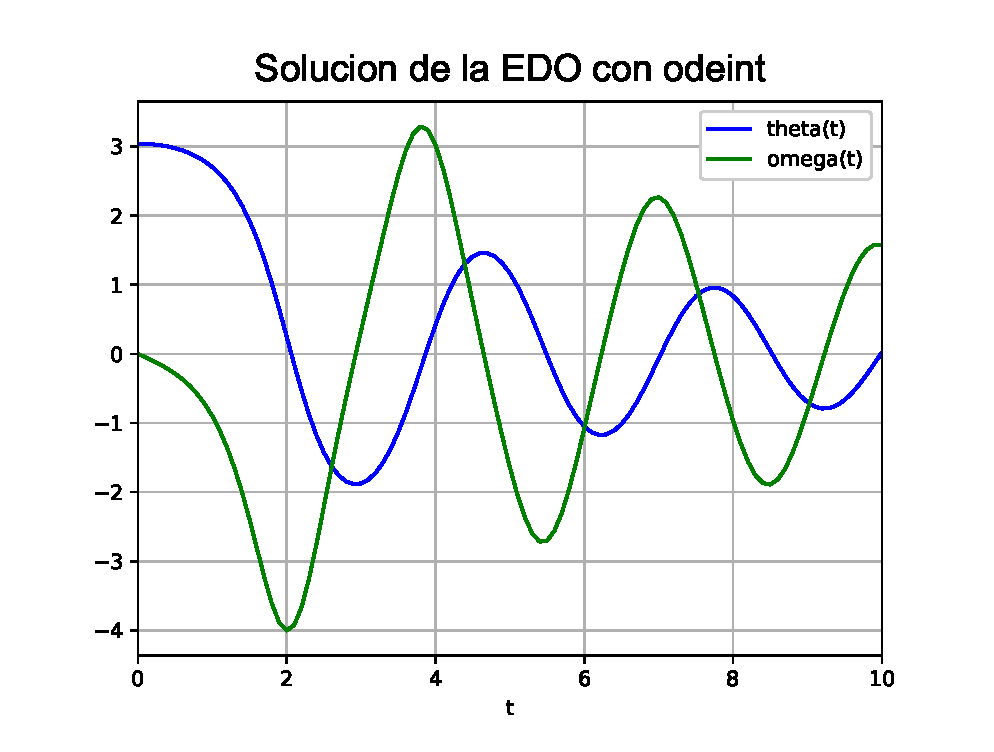
\includegraphics[scale=0.5]{Imagenes/sol_odeint_01.eps}
% \end{figure}
% \end{frame}
% \begin{frame}
% \frametitle{Gráfica del espacio fase}
% La segunda gráfica representa el espacio fase, y como podemos ver, hay un atractor debido a la fricción en el péndulo.
% \begin{figure}
%     \centering
%     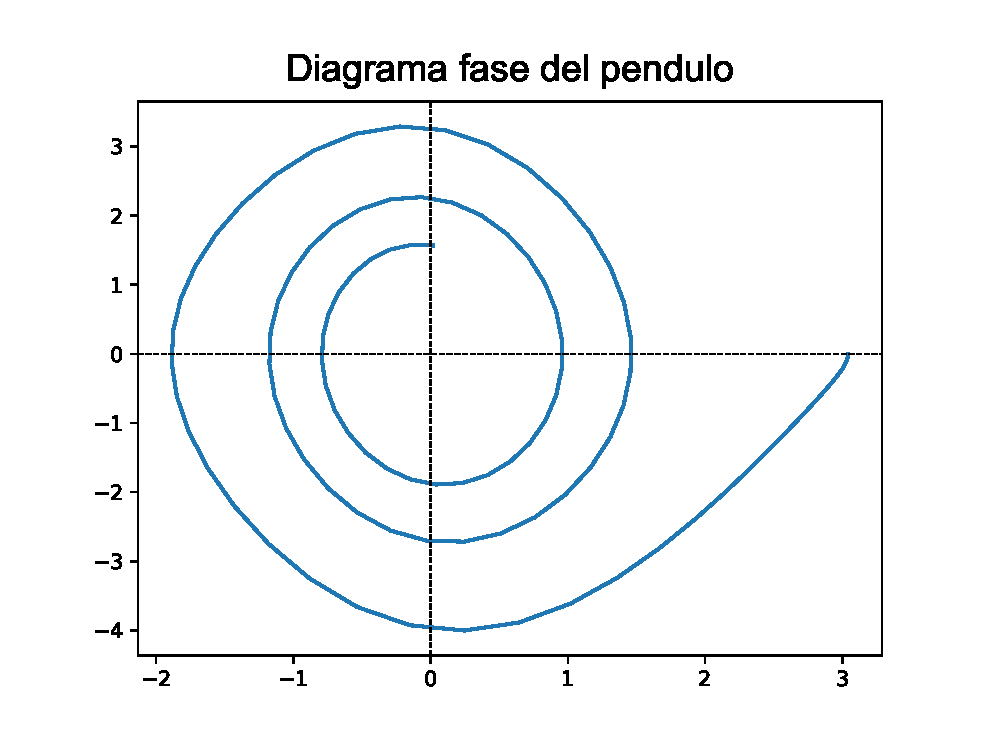
\includegraphics[scale=0.5]{Imagenes/sol_odeint_02.eps}
% \end{figure}
% \end{frame}
% \begin{frame}
% \frametitle{Ejercicio 2}
% La ecuación de movimiento para el oscilador amortiguado es:
% \[ \dfrac{d^{2} x}{dt^{2}} + 2 \: \zeta \:  \omega_{0} \dfrac{dx}{dt} + \omega_{0}^{2} \: x = 0\]
% donde $x$ es la posición del oscilador, $\omega_{0}$ la frecuencia, y $\zeta$ es el factor de amortiguamiento.
% \end{frame}
% \begin{frame}
% Para escribir esta \textoazul{2-EDO} en la forma estándar, introducimos $p = dx/dt$
% \begin{align*}
% \dfrac{dp}{dt} &= - 2 \: \zeta \: \omega_{0} \: p - \omega^{2} \: x \\
% \dfrac{dx}{dt} &= p
% \end{align*}
% \end{frame}
% \begin{frame}
% Veremos con este ejemplo, la versatilidad de pasar argumentos extras a la función, que representan diferentes valores del factor de amortiguamiento.
% \\
% \bigskip
% De tal manera que en una sola ejecución del código, podemos realizar el pase de valores, de otra manera, tendríamos que realizar una ejecución del código y modificar a mano el valor del factor de amortiguamiento.
% \end{frame}
% \begin{frame}
% Como consecuencia de los argumentos extra, necesitamos pasar un argumento clave \texttt{args} a la función \azulfuerte{\texttt{odeint}}.
% \\
% \bigskip
% $\zeta = 0.0, 0.2, 1.0, 5.0 $
% \end{frame}
% \begin{frame}[plain, allowframebreaks, fragile]
% \frametitle{Código para resolver el problema}
% \begin{lstlisting}[caption=Código completo, style=FormattedNumber, basicstyle=\linespread{1.1}\ttfamily=\small, columns=fullflexible]
% from scipy.integrate import odeint
% from numpy import zeros, array, linspace
% import matplotlib.pyplot as plt

% def F(y, t, zeta, w!0!):
%     F = zeros((2), dtype='float!6!!4!')
%     F[!0!] = y[!1!]
%     F[!1!] = -2 * zeta * w!0! * y[!1!] - w!0!**2 * y[!0!]
%     return F    

% y!0! =array([1.0, 0.0])

% t = linspace(0, 10, 1000)
% w!0! = 2*pi*1.0


% y!1! = odeint(F, y!0!, t, args=(0.0, w!0!))
% y!2! = odeint(F, y!0!, t, args=(0.2, w!0!))
% y!3! = odeint(F, y!0!, t, args=(1.0, w!0!))
% y!4! = odeint(F, y!0!, t, args=(5.0, w!0!))

% plt.axis([0, 10, -1.05, 1.05])
% plt.plot(t, y!1![:,!0!], 'k', label="no amortiguado")
% plt.plot(t, y!2![:,!0!], 'r', label="subamortiguado")
% plt.plot(t, y!3![:,!0!], 'b', label="amortiguado critico")
% plt.plot(t, y!4![:,!0!], 'g', label="sobreamortiguado")
% plt.legend()
% plt.show()
% \end{lstlisting}
% \end{frame}
% \begin{frame}[fragile]
% \frametitle{Resultado}
% \begin{figure}
%     \centering
%     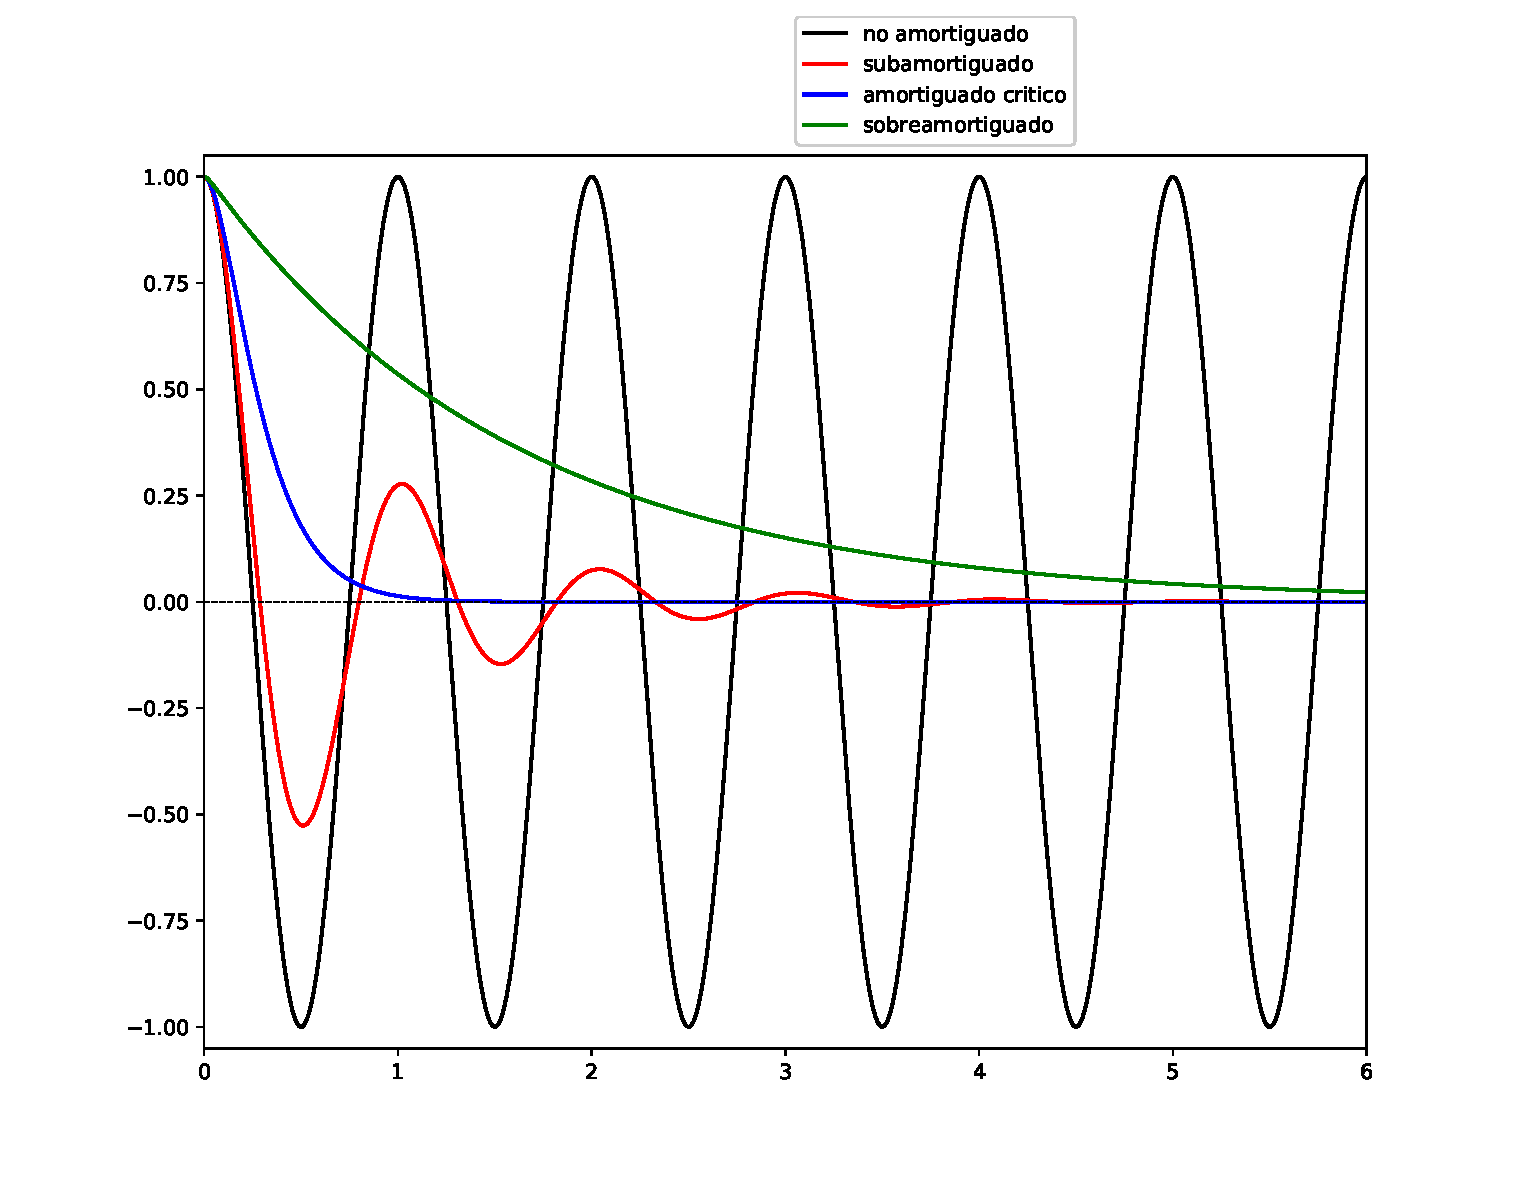
\includegraphics[scale=0.4]{Imagenes/sol_odeint_03.eps} 
% \end{figure}
% \end{frame}
\end{document}